\documentclass[11pt]{amsart}

% Margins
\usepackage[headheight=65pt]{geometry}
\geometry{
  top=1 in,
  inner=1 in,
  outer=1 in,
  bottom=1 in,
  headheight=3ex,
  headsep=2ex,
}

% Personal info, class, assignment
\def \fnamea{Dennis}
\def \fnameb{Neill}
\def \lnamea{Windham}
\def \lnameb{Shikada}
\def \class{CSCI 5448}
\def \hwnum{7} % Homework number
\def \assgn{Project \hwnum}
\newif\ifcode % Switch to toggle Python code insertion, see the end of the document for the value assignment

% Header
\usepackage{fancyhdr}
\pagestyle{fancy}
\lhead{\lnameb\ \& \lnamea}
\fancyfoot{}
\chead{\assgn}
\rhead{Page \thepage}
\renewcommand{\headrulewidth}{2pt}
%\renewcommand{\footrulewidth}{1pt}
\usepackage{pdflscape}


\usepackage{enumitem}
\usepackage{tabularx}
\usepackage{amssymb,amsmath,amsthm,amscd,mathrsfs,graphicx,color,pdfpages}
\usepackage[cmtip,all,matrix,arrow,tips,curve]{xy}
\usepackage[active]{srcltx}
\usepackage{mathpazo}
\usepackage{setspace}\doublespacing 
%Double space, and make it easier for the grader to grade your homework.
\usepackage{hyperref}
\usepackage[usenames,dvipsnames]{xcolor}
\usepackage[style=science,sortcites=true,sorting=nyt,backend=biber]{biblatex}
\hypersetup{colorlinks=true,citecolor=ForestGreen,linkcolor=Maroon,urlcolor=NavyBlue}

% Python raw code insertion
\usepackage{listings}
\usepackage{color}

% Python linting settings
\definecolor{dkgreen}{rgb}{0,0.6,0}
\definecolor{gray}{rgb}{0.5,0.5,0.5}
\definecolor{mauve}{rgb}{0.58,0,0.82}
\lstset{frame=tb,
  language=Python,
  aboveskip=3mm,
  belowskip=3mm,
  showstringspaces=false,
  columns=flexible,
  basicstyle={\small\ttfamily},
  numbers=none,
  numberstyle=\tiny\color{gray},
  keywordstyle=\color{blue},
  commentstyle=\color{dkgreen},
  stringstyle=\color{mauve},
  breaklines=true,
  breakatwhitespace=true,
  tabsize=3
}

% References
\addbibresource{./references.bib}

% Allows vertical lines in matrices like in tables
% Usage:
% \begin{bmatrix}[cc|cc] ...
\makeatletter
\renewcommand*\env@matrix[1][*\c@MaxMatrixCols c]{%
  \hskip -\arraycolsep
  \let\@ifnextchar\new@ifnextchar
  \array{#1}}
\makeatother

\newcommand{\marg}[1]{\normalsize{{\color{blue}\footnote{{\color{blue}#1}}}{\marginpar[\vskip -.3cm {\color{blue}\hfill\thefootnote$\implies$}]{\vskip -.3cm{ \color{blue}$\impliedby$\thefootnote}}}}}

\newcommand{\qc}[1]{\marg{#1}}

\setlength\fboxsep{.3cm}
\setlength\fboxrule{.05cm}

% Custom boxes
\newcommand*{\boxedcolor}{orange}
\makeatletter
\renewcommand{\boxed}[1]{\textcolor{\boxedcolor}{%
  \fbox{\normalcolor\m@th$\displaystyle#1$}}}
\makeatother

\makeatletter
\newcommand{\boxedred}[1]{\textcolor{red}{%
  \fbox{\normalcolor\m@th$\displaystyle#1$}}}
\makeatother

\makeatletter
\newcommand{\boxedblue}[1]{\textcolor{blue}{%
  \fbox{\normalcolor\m@th$\displaystyle#1$}}}
\makeatother

% Begin Document
\begin{document}

%region Author, Title, Abstract, TOC
\author[\lnamea]{\fnamea\ \lnamea\\\fnameb\ \lnameb}
\date{\today}
\title[\assgn]{\assgn \\ \ \\\class}
\maketitle
\tableofcontents
%endregion

\newpage
\section*{\textbf{Final Project Report}}
\subsection*{Title}
\begin{center}
    \textit{Object Oriented Civilization Game Clone}
\end{center}

\subsection*{Team Members} \phantom{}

\begin{table}[htbp]
    \begin{tabularx}{\textwidth}{l|l|l}
        \textbf{Name}    & \textbf{Role}    & \textbf{Email}                  \\
        \hline
        Neill Shikada    & Graduate Student & Neill.Shikada@colorado.edu
        \\
        Dennis Windham   & Graduate Student & dene5275@colorado.edu           \\
        Bruce Montgomery & Instructor       & bruce.r.montgomery@colorado.edu
    \end{tabularx}
\end{table}

\subsection*{Final State of System Statement}
We were able to implement most of the proposed functionality.
\begin{itemize}
    \item There is a complete board with 3D models.
    \item There are four distinct players on the game board, three being AI-controlled and one human-controlled.
    \item The AI makes decisions on its own regarding how to spawn and move units.
    \item The player can move units with arrow keys and spawn with number keys.
    \item Player-controlled units correctly detect cells they can't move into, attack selected targets or move into free cells.
    \item The player can spawn units with number keys ($1,2,3$).
\end{itemize}

What wasn't implemented implemented:
\begin{itemize}
    \item We wanted to give the project more visual fidelity, but had to cut down on this aspect due to time constraints.
    \item We wanted to implement end-game statistics, but couldn't find time for it due to a heavy workload in other classes.
\end{itemize}

Project 5 was a design submission, and our goals or design elements did not really change. Project 6 was almost a complete submission of the project, and since then we dialed in some AI elements and added human controls.

\newpage
\subsection*{Final Class Diagram and Comparison Statement} \phantom{}

% •
%  A thorough UML class diagram representing your final set of classes and key relationships of the
% system
% •
%  Highlight and document in that diagram any patterns that were included (in whole or part) in your
% design
% •
%  Include the class diagram submitted in Project 5, and use it to show what changed in your system
% from that point into the final submission
% •
%  Support the diagrams with a written paragraph identifying key changes in your system since your
% design/work was submitted in Projects 5 and 6




See \hyperref[sec:appendixa]{Appendix A: Demonstration Class Diagram} for our class diagram.

\subsection*{Third-Party code vs. Original code Statement} \phantom{}

We are using the Unity3D game engine for this project. However, we purposely limited involvement of Unity's bloated \texttt{MonoBehavior} class. It is conventional for Unity developers to have every class in the program inherit from \texttt{MonoBehavior}, but we are keeping the overwhelming majority of our code pure \texttt{C\#}, and where possible use the adapter pattern to interact with \texttt{MonoBehavior}. 

\subsection*{Statement on the OOAD process for your overall Semester Project} \phantom{}
% List three key design process elements or issues (positive or negative) that your team experienced in
% your analysis and design of the OO semester project

\begin{enumerate}
    \item[(1)] Throughout the development of the project, we held biweekly meetings lasting anywhere from 18 to 24 hours. During out meetings, we primarily discussed the state of our project, design approaches to consider moving forward and how OO patterns could solve the problems we envisioned. This level of dedication secured a robust design for our project early on and helped us stay on track during development. 
    \item[(2)] A major part of our design process was sticking at least to the following OO principles:
    \begin{itemize}
        \item Program to an interface, not implementation
        \item Encapsulate what varies
        \item Favor composition over inheritance
        \item Aim for loose coupling, strong cohesion
        \item Single Responsibility Principle
        \item Open-Closed Principle
        \item Liskov Substitution Principle
    \end{itemize}

    Generally speaking, it worked well for us, although we cannot state with absolute certainty that none of our code violates the said principles. However, we feel that we still managed to write a rather clean and maintainable codebase. 
    
    \item[(3)]
    
    We felt that as our project grew, the readability of its UML class diagram greatly deteriorated. In fact, at one point, after an intense coding session which involved inclusion of a number of unforeseen classes, we were flabbergasted to find out that the new class diagram looked twice as convoluted as before.


\end{enumerate}

% create a new page with special dimensions, include diagram
\newpage
\paperwidth=30in
\paperheight=20in
\pdfpagewidth=\paperwidth
\pdfpageheight=\paperheight

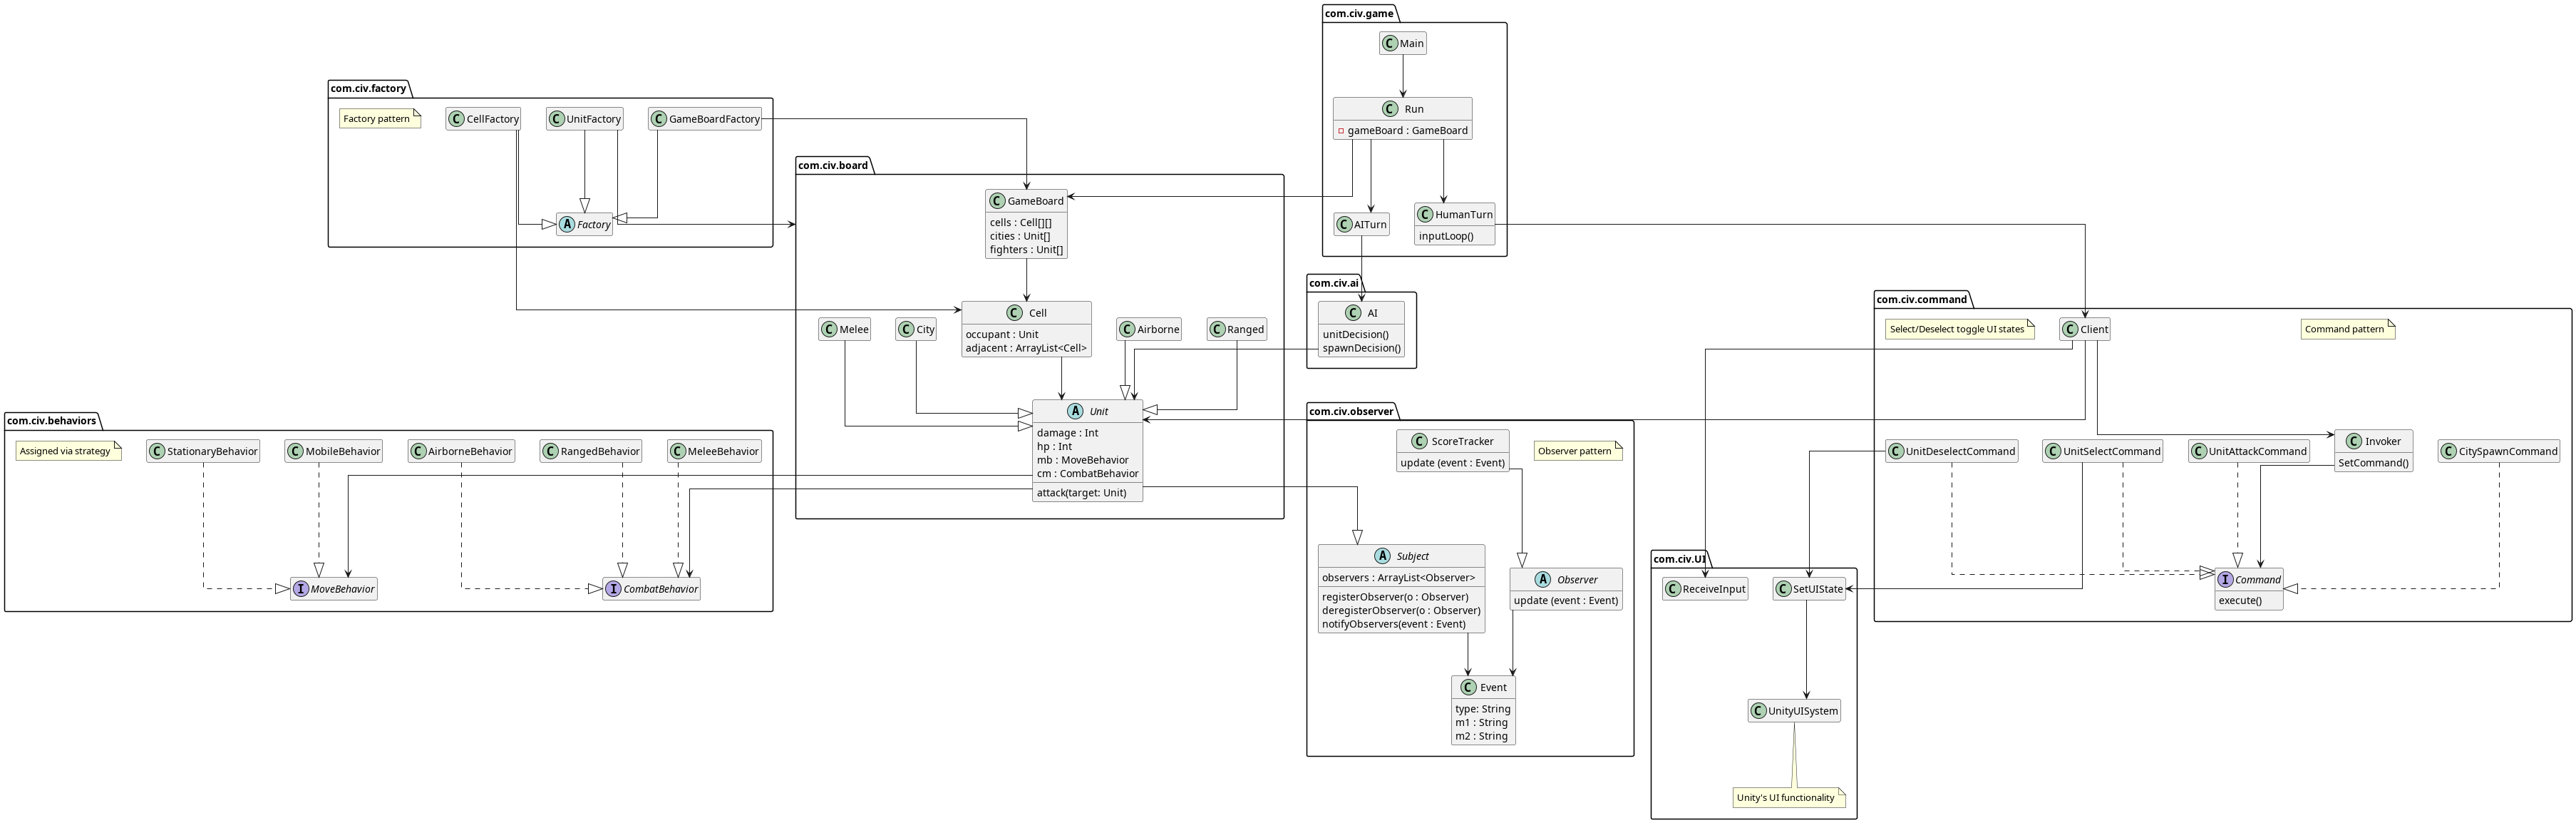
\includepdf[scale=0.9, offset=0mm 0mm, pagecommand={\section*{Appendix A: Demonstration Class Diagram}\pagestyle{fancy}}\label{sec:appendixa}]{../diagrams/class/class.png}


%\codetrue % Uncomment to enable code insertion
\ifcode
    % Python code section, toggled by the switch above
    % The code file is expected to be follow the "hw{\hwnum}.py" naming convention
    \newpage
    \section*{Code}
    \label{sec:code}
    \lstinputlisting[language=Python]{Code/hw\hwnum.py}
\fi


% \includepdf[scale=0.98, pagecommand={\section*{Appendix A: Class Diagram for RotLA}\pagestyle{fancy}}\label{sec:appendixa}]{../uml/game_diagram.png}


\end{document}
